\documentclass[aspectratio=169]{beamer}
%[handout]

\usetheme[progressbar=frametitle]{metropolis}
\usepackage{appendixnumberbeamer}

\usepackage[utf8]{inputenc}
\usepackage[T1]{fontenc}

\usepackage[brazil]{babel}
\usepackage[outputdir=..]{minted}
\usepackage{xcolor}
\usepackage{soul} % strikethrough
\usepackage{advdate}
\usepackage{graphicx}
\graphicspath{{figs/}}
\usepackage{graphbox}

\usepackage[ampersand]{easylist}

\usepackage{multirow}
\usepackage{multicol}
\usepackage{subcaption}

\usepackage{pgf,tikz}
\usetikzlibrary{shapes,arrows,positioning}
\usetikzlibrary{circuits.logic.US}
\usetikzlibrary{matrix,calc}

\usepackage{karnaugh-map}

\usepackage{pgfpages}
\setbeameroption{hide notes} % Only slides
% \setbeameroption{show only notes} % Only notes
% \setbeameroption{show notes on second screen=right} % Both

% \graphicspath{{../figs/}}

\definecolor{bgc}{rgb}{0.95,0.9,0.95}
\definecolor{links}{HTML}{2A7F7F}
\hypersetup{colorlinks,linkcolor=,urlcolor=links}

\newminted{verilog}{fontsize=\scriptsize, 
    linenos,
    numbersep=8pt,
    bgcolor=bgc,
    tabsize=4,
    framesep=3mm} 
    %frame=lines,

\newcommand{\verilog}[1]{\verilogf{#1}{\footnotesize}}

\newcommand{\verilogf}[2]{\inputminted[fontsize=#2, 
    linenos,
    tabsize=2,
    numbersep=4pt,
    bgcolor=bgc,
    framesep=3mm]{verilog}{../codes/#1.v}
}

\newminted{nasm}{fontsize=\scriptsize, 
		   linenos,
		   numbersep=8pt,
           bgcolor=bgc,
		   framesep=3mm} 

\usepackage{booktabs}
\usepackage[scale=2]{ccicons}

\usepackage{pgfplots}
\usepgfplotslibrary{dateplot}

\usepackage{hyperref}


\usepackage{xspace}
\newcommand{\themename}{\textbf{\textsc{metropolis}}\xspace}



\usepackage{pifont}% http://ctan.org/pkg/pifont
\newcommand{\cmark}{\ding{51}}%
\newcommand{\xmark}{\ding{55}}%

% \tiny	
% \scriptsize
% \footnotesize
% \small	
% \normalsize	
% \large	
% \Large	
% \LARGE	
% \huge	
% \Huge	



\newminted{python}{fontsize=\scriptsize, 
		   linenos,
		   breaklines,
		   numbersep=8pt,
           tabsize=2,
		   framesep=3mm} 
		   
\newminted{verilog}{fontsize=\scriptsize, 
		   linenos,
		   breaklines,
		   numbersep=8pt,
           tabsize=2,
		   framesep=3mm} 
		   




\definecolor{bgc}{rgb}{0.95,0.9,0.95}
\definecolor{links}{HTML}{2A7F7F}
\hypersetup{colorlinks,linkcolor=,urlcolor=links}


% \usepackage[style=apa]{biblatex}
% \addbibresource{mm.bib}


% \author{\large Prof. Ricardo Menotti (\href{mailto:menotti@ufscar.br}{menotti@ufscar.br})}

\newcommand{\newauthor}[2]{
  \parbox{0.50\textwidth}{
    \texorpdfstring
      {
        \centering
        \small #1 \newline
        {\scriptsize{\urlstyle{same}\href{mailto:#2}{#2}\urlstyle{tt}}}
      }
      {#1} \newline
  }
}

\author{
  \newauthor{Prof. Ricardo Menotti}{menotti@ufscar.br}
\and \newauthor{Prof. Luciano de Oliveira Neris}{lneris@ufscar.br}  
%\and \newauthor{Prof. Artino Quintino da Silva Filho}{artino@ufscar.br}
% \and \newauthor{Prof. Maurício Figueiredo}{mauricio@ufscar.br}
% \and \newauthor{Prof. Edilson Kato}{kato@ufscar.br}
% \and \newauthor{Prof. Roberto Inoue}{rsinoue@ufscar.br}
}

\date{Atualizado em: \today}

\institute{\large \textbf{Departamento de Computação} \\
Centro de Ciências Exatas e de Tecnologia \\
Universidade Federal de São Carlos}

\title{Lógica Digital (1001351)}

\titlegraphic{\hfill
\includegraphics[height=1.5cm]{LogoUfscar}}



\subtitle{Introdução à Verilog} % 

\begin{document}

\begin{frame}
	\titlepage
\end{frame} 

\section{Introdução à Verilog}

\begin{frame}{\insertsection} % Slide with bullets
	\begin{itemize}
		\item Verilog é uma linguagem complexa, mas neste curso não vamos abordar todas as suas potencialidades;
		\item O que vamos aprender será suficiente para projetar e testar uma grande variedade de circuitos;
		\item Iremos abordar as funcionalidades da linguagem a medida que avançarmos com os circuitos digitais; 
		\item A principal habilidade desejada neste curso é a capacidade de traduzir com facilidade um circuito para Verilog e vice-versa; 
		\item Isso só pode ser alcançado com a prática, pois assim como na programação, estudar problemas resolvidos não ajuda muito. 
    \end{itemize}
\end{frame}

\begin{frame}{\insertsection} % Slide with bullets
	\begin{itemize}
		\item Em Verilog há várias maneiras de se descrever um mesmo circuito, por exemplo, a partir:
		\begin{itemize}
			\item \textbf{Funcional ou Lógica:} de funções ou portas básicas; 
			\item \textbf{Estrutural:} de uma hierarquia de componentes; 
			\item \textbf{Comportamental:} da descrição de seu comportamento; 
		\end{itemize}
		\item Pode-se usar combinações das metodologias. 
	\end{itemize}
\end{frame}

\begin{frame}[fragile]{Exemplo: multiplexador} % Slide with bullets
     \begin{columns}
         \begin{column}{0.50\textwidth}
			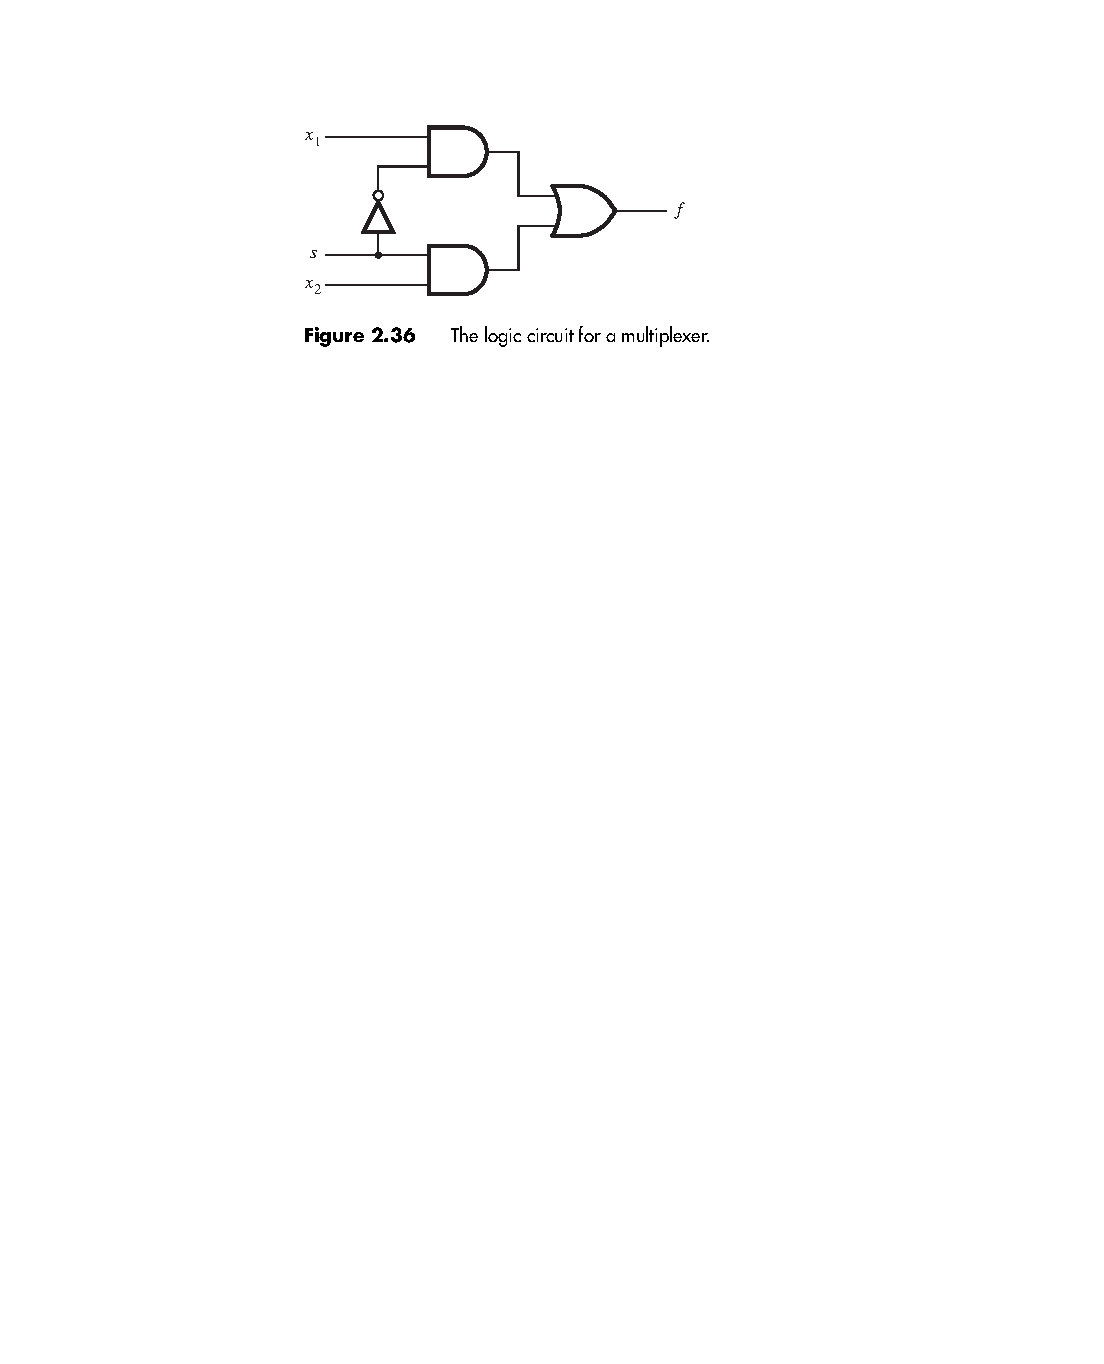
\includegraphics[width=\textwidth]{VerilogFig2_36}
	\begin{verilogcode}
// Behavioral specification
module example3(input x1, x2, s,
                output reg f); 
  always @(x1, x2, s)
    if (s==0)
      f = x1;
    else
      f = x2;
endmodule
	\end{verilogcode} 
         \end{column}
         \begin{column}{0.50\textwidth}
	\begin{verilogcode}
module example2(input x1, x2, s,
                output f); 
  assign f = 
         (x1 & ~s) | (x2 & s); 
endmodule
	\end{verilogcode} 
	\begin{verilogcode}
module example1(x1, x2, s, f); 
  input x1, x2, s;
  output f;

  not (k, s); 
  and (g, k, x1);
  and (h, s, x2); 
  or (f, g, h);
endmodule
	\end{verilogcode} 
         \end{column}        
     \end{columns}
\end{frame}

\begin{frame}[fragile]{Outro exemplo}
     \begin{columns}
         \begin{column}{0.55\textwidth}
	\begin{verilogcode}
module example2 (x1, x2, x3, x4, f, g, h); 
  input x1, x2, x3, x4;
  output f, g, h;

  and (z1,  x1,  x3); 
  and (z2,  x2,  x4); 
  or  (g,   z1,  z2);
  or  (z3,  x1, ~x3); 
  or  (z4, ~x2,  x4); 
  and (h,   z3,  z4); 
  or  (f,    g,   h);
endmodule
	\end{verilogcode} 
	\vspace{-0.1cm}
	\begin{verilogcode}
module example2 (x1, x2, x3, x4, f, g, h); 
  input x1, x2, x3, x4;
  output f, g, h;

  assign g = (x1 & x3)|(x2 & x4); 
  assign h = (x1 | ~x3)&(~x2 | x4);
  assign f = g | h;
endmodule
	\end{verilogcode} 
         \end{column}
         \begin{column}{0.45\textwidth}
			\hspace*{-14pt}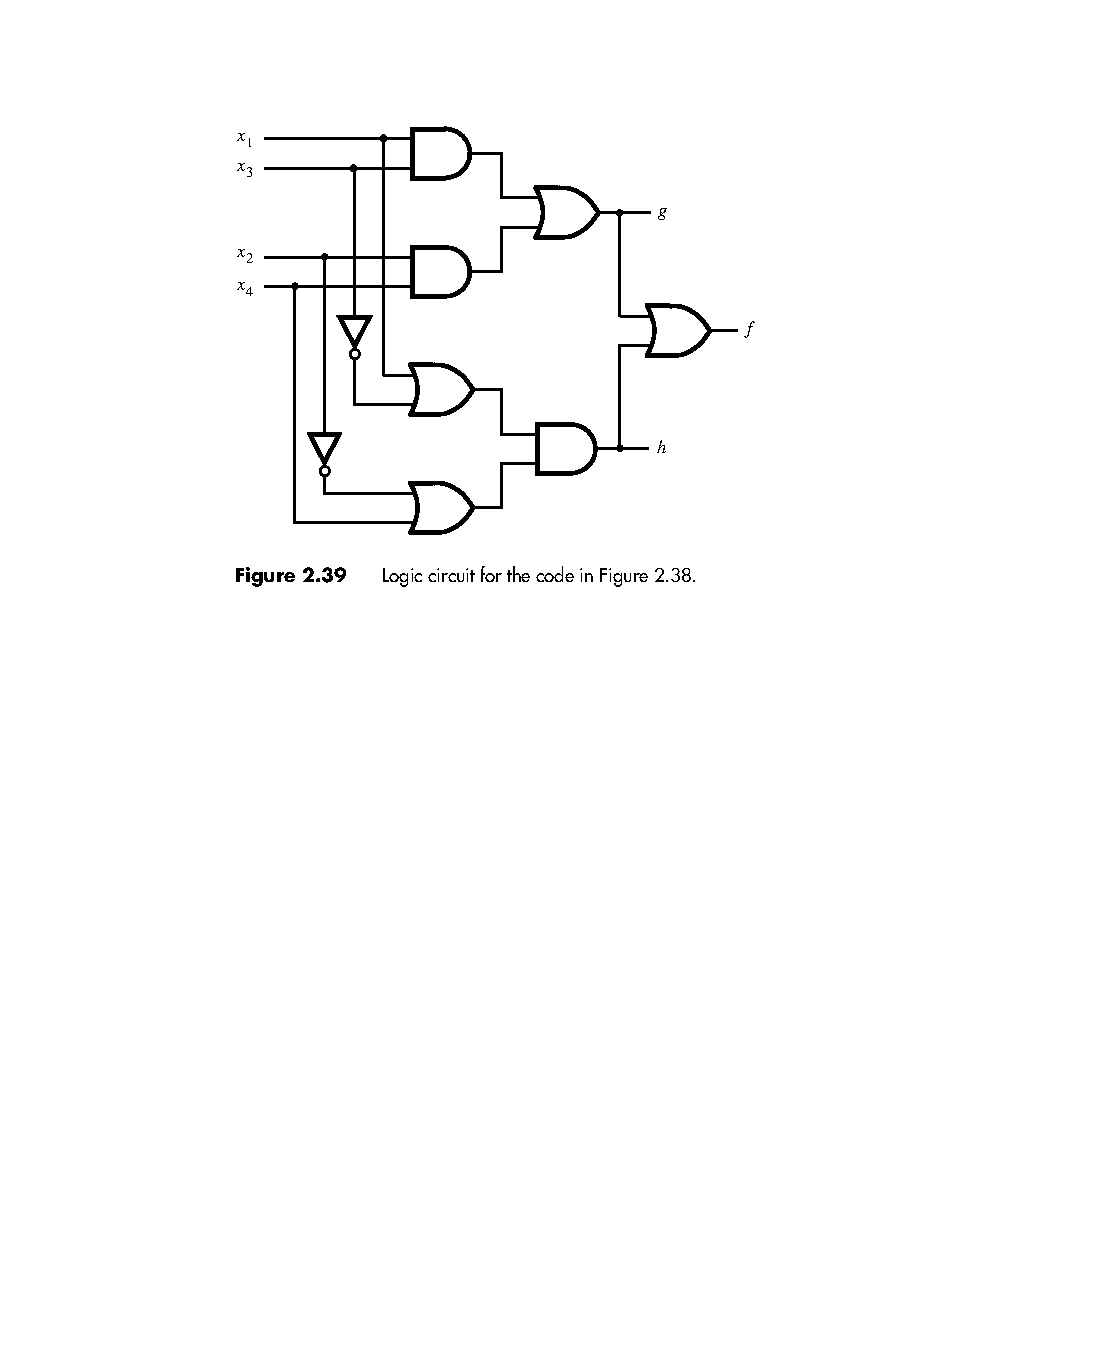
\includegraphics[width=1.2\textwidth]{VerilogFig2_39}
         \end{column}        
     \end{columns}
\end{frame}

 \begin{frame}{\insertsection} \centering
     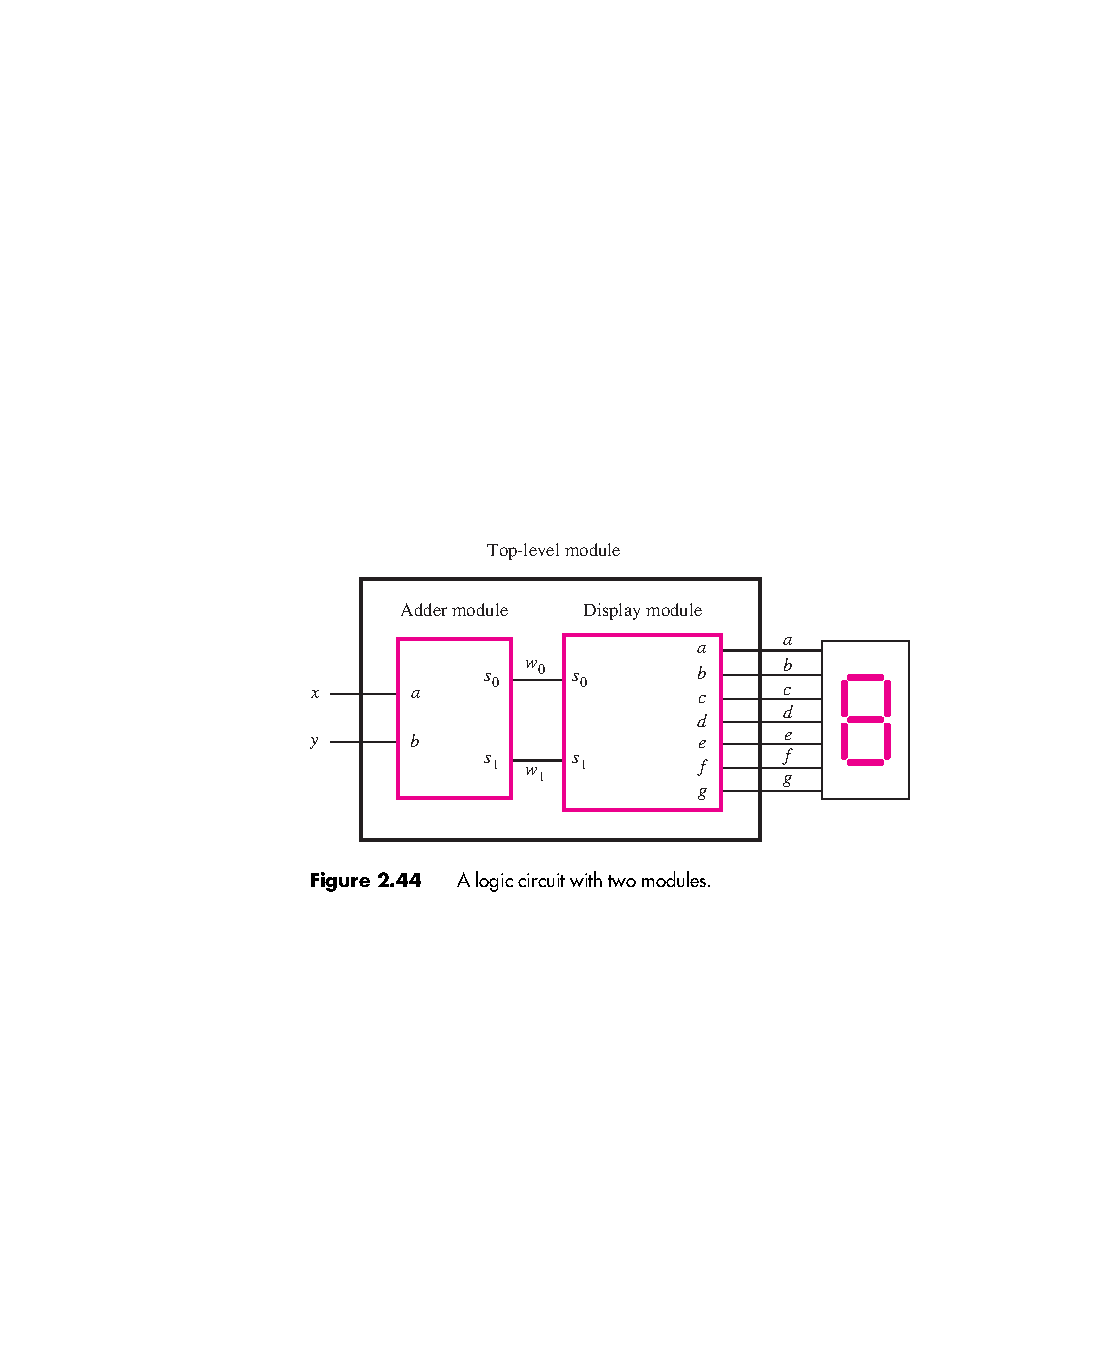
\includegraphics[width=.9\textwidth]{VerilogFig2_44}
 \end{frame}

\begin{frame}[fragile]
	\frametitle{\insertsection}
     \begin{columns}
         \begin{column}{0.52\textwidth}
	\begin{verilogcode}
// Top-level module
module adder_display(x, y, a, b, 
                 c, d, e, f, g); 
  input x, y;
  output a, b, c, d, e, f, g; 
  wire w1, w0;

  adder U1 (x, y, w1, w0);
  display U2 (w1, w0, a, b, c, 
              d, e, f, g);
endmodule
	\end{verilogcode} 
	\begin{verilogcode}
// An adder module
module adder (a, b, s1, s0);
  input a, b; 
  output s1, s0;

  assign s1 = a & b; 
  assign s0 = a ^ b;
endmodule
	\end{verilogcode} 
         \end{column}
         \begin{column}{0.48\textwidth}
	\begin{verilogcode}
// A module for driving a 
//      7-segment display 
module display(s1, s0, a, b, 
               c, d, e, f, g);
  input s1, s0;
  output a, b, c, d, e, f, g;

  assign a = ~s0;
  assign b = 1;
  assign c = ~s1;
  assign d = ~s0;
  assign e = ~s0;
  assign f = ~s1 & ~s0;
  assign g = s1 & ~s0;
endmodule
	\end{verilogcode} 
         \end{column}        
     \end{columns}
\end{frame}

\begin{frame}{Como NÃO escrever Verilog}
    \begin{itemize}
        \item NÃO escrever código que se assemelhe a um programa de computador, contendo muitas variáveis e loops; 
        \begin{itemize}
            \item É difícil determinar qual circuito lógico as ferramentas CAD produzirão ao sintetizar código assim;
        \end{itemize}
        \item Neste curso veremos exemplos completos de código Verilog que representam uma ampla gama de circuitos lógicos; 
        \begin{itemize}
            \item Neles o código é facilmente relacionado ao circuito lógico descrito;
            \item Procure adotar o mesmo estilo de código;
        \end{itemize}
        \item \emph{Se não for possível determinar prontamente qual circuito lógico é descrito pelo código Verilog, então as ferramentas CAD provavelmente não sintetizarão o circuito que o projetista está tentando modelar;}
        \item \textbf{Analise o circuito resultante produzido pelas ferramentas de síntese; }
    \end{itemize}
\end{frame}

\section{Bibliografia} %%%%%%%

\begin{frame}{\insertsection} 
	\begin{itemize}
		\item \href{https://www.google.com.br/search?q=filetype\%3Apdf+Fundamentals+of+Digital+Logic+with+Verilog+Design+&oq=filetype\%3Apdf}{Brown, S. \& Vranesic, Z. - Fundamentals of Digital Logic with Verilog Design, 3rd Ed., Mc Graw Hill, 2009}
		\item \href{http://www.asic-world.com/verilog/}{http://www.asic-world.com/verilog/}
		\item \href{https://www.edaplayground.com/}{https://www.edaplayground.com/}
            \item \url{https://digitaljs.tilk.eu/}
	\end{itemize}
\end{frame}

\begin{frame}
	\titlepage
\end{frame} 

\end{document}